\documentclass[a4paper,12pt,reqno]{article}

\usepackage{styledoc19}


\begin{document} % конец преамбулы, начало документа
	
	
	\year{2021}
    \docNumber{RU.17701729.09.09-62 ТЗ 01-1}
	\docFormat{Техническое задание}
	\student{БПИ 174}{Д. Ю. Редникина}
	
	\project{CRM-СИСТЕМА ДЛЯ БЛАГОТВОРИТЕЛЬНОГО ФОНДА <<AIAIN>>. WEB-ПРИЛОЖЕНИЕ ДЛЯ СОТРУДНИКОВ ФОНДА}
	

	\supervisor{Доцент департамента \vfill образовательной программы  \vfill <<Программная инженерия>>}
	{Х. М. Салех}
	
	\firstPage
						\newpage
	\secondPage
						\newpage
	\thirdPage
						\newpage
	\section{Введение}
	\subsection{Наименование программы}
	\subsubsection{Наименование программы на русском языке}
	CRM-система для благотворительного фонда <<AIAIN>>. Web-приложение для сотрудников фонда
	\subsubsection{Наименование программы на английском языке}
	System for managing tasks of collecting data from the Internet

	\subsection{Краткая характеристика области применения}
	Ежегодно сотни тысяч людей жертвуют свои деньги некоммерческим организациям. Еще больше людей обращаются за помощью в общественные благотворительные фонды. Управлять благотворительным фондом становится все сложнее. Нужно не только принимать пожертвования и регистрировать заявки на сборы средств, но и контролировать работников фонда, волонтеров, подготавливать документацию для вышестоящих органов и многое другое. 

Следовательно, некоммерческие организации нуждаются в платформе с функционалом, ориентированным на бизнес процессы фонда, чтобы обрабатывать всю необходимую информацию в одном месте. К сожалению, большинство фондов пользуются электронными таблицами или, что еще хуже, ведут записи в бумажной форме. Как результат, на каждое действие тратятся большое количество времени и ресурсов. Арабский фонд <<AIAIN>> также столкнулся с проблемой автоматизации бизнес процессов, специфичных для предметной области благотворительности. 


Разрабатываемое Web-приложение ориентировано на специфические нужды некоммерческой организации <<AIAIN>>. Web-приложение для сотрудников фонда может предоставить все преимущества, которыми бизнес-компании пользовались в течение многих лет и чего так не хватало этому фонду. Это также позволит наладить бизнес-процессы внутри фонда <<AIAIN>>, настроить тайм-менеджмент и автоматизировать составление отчетности.
	\newpage
	\section{Основания для разработки}
	\subsection{Документы, на основании которых ведется разработка}
	
	
	Приказ декана факультета компьютерных наук И.В. Аржанцева "Об утверждении тем, руководителей курсовых работ студентов образовательной программы «Программная инженерия» факультета компьютерных наук" № 2.3-02/1112-04 от 11.12.2019.
	
	\subsection{Наименование темы разработки}
	
	Наименование темы разработки – <<CRM-система для благотворительного фонда <<AIAIN>>. Web-приложение для сотрудников фонда>> (<<System for managing tasks of collecting data from the Internet
>>)


 Программа выполняется в рамках темы выпускной квалификационной работы в соответствии с учебным планом подготовки бакалавров по направлению 09.03.04 «Программная инженерия» Национального исследовательского университета «Высшая школа экономики», факультет компьютерных наук.
	
	\newpage 
	\section{Назначение разработки}
	 
	\subsection{Функциональное назначение}
	Система будет применяться как средство управления проектами по созданию, редактированию и запуску веб краулеров для сбора данных в сети интернет. Продукт позволит следить за запусками в режиме реального времени, а также создавать периодические запуски по расписанию.

	\subsection{Эксплуатационное назначение}
	Web-приложение является компонентом CRM-системы для благотворительного фонда <<AIAIN>>, позволяющей облегчить бизнес процессы работы фонда с благополучателями и донорами. Web-приложение призвано обеспечить необходимую сотрудникам фонда функциональность для работы с системой. Им будут пользоваться как менеджеры фонда, так и администраторы, члены комиссий, операторы фонда, контент-менеджеры фонда. Каждый из пользователей будет иметь доступ к необходимой ему функциональности по обработке заявок, управлению фондом, администрированию и т.д. 
	
						\newpage
	\section{Требования к программе}
	
	\subsection{Функциональные требования}
	
	Клиентская часть для сотрудников фонда <<AIAIN>> должна быть реализована в виде веб-приложения, запускаемого в браузере, и представлена в виде интерфейса для CRM-системы для благотворительного фонда <<AIAIN>>. Клиентское приложение должно предоставлять функционал для сотрудников фонда по управлению заявками на сбор средств, просмотром поступивших средств, управлению контентом фонда, администрированию сотрудников. 
	
	Требования к клиентскому приложению были составлены в соответствии с диаграммой прецедентов, которая представлена в Приложении \ref{usecaseWeb}.

    \newlist{subreg}{enumerate}{10}
 
\setlist[subreg, 1]{label=\textbf{FR-\arabic*.}}
\setlist[subreg, 2]{label*=\textbf{\arabic*.}}
\setlist[subreg, 3]{label=\arabic*.}

\begin{subreg}
    \item \label{FR-1} \textbf{Аутентификация\\} 
	Сотрудник фонда должен иметь возможность авторизоваться в системе с логином/паролем, предварительно полученным после регистрации по почте. Процесс регистрации и получения логина/пароля описан в пункте \ref{enum:reg}. Если пользователь не зарегистрирован в системе или авторизуется с неверными данными, то система должна отобразить соответствующее сообщение. 
	
	При первоначальном авторизации в системе на новом устройстве пользователь должен увидеть диалоговое окно с возможностью принять или отклонить получение пуш-уведомлений (подробнее о пуш-уведомлениях в разделе \ref{push}).
	
	\item \textbf{Настройки\\}
    У пользователя должна быть возможность управлять личными данными в настройках системы.
    \begin{subreg} \label{settings}
        \item Должна быть возможность просмотра информации о своем профиле в настройках системы:
        \begin{subreg}
        \item ФИО, почта;
        \item Дата рождения;
        \item Город, страна, телефон;
        \item Фотография;
        \item Роль в системе (см. Приложение \ref{stuff});
        \item Назначенные категории (только для пользователей с ролью <<Член комиссии>>);
        \end{subreg}
        \item Должна быть возможность изменения основной информации:
    \begin{subreg}
        \item ФИО;
        \item Город, страна, телефон;
        \item Фотография;
        \item Дата рождения;
    \end{subreg}
        \item Должна быть возможность выбрать язык системы: русский или английский;
        \item \label{enum:push} Должна быть возможность включить/отключить получение пуш-уведомлений; 
    \end{subreg}
    \item \textbf{Пуш-уведомления\\} \label{push}
    Сотрудники фонда должны иметь возможность получать пуш-уведомления, если такая настройка включена (см. пункт \ref{enum:push}).
    
    \begin{subreg}
        \item Должна быть возможность получения пуш-уведомлений на входящие сообщения в чатах поддержки (для пользователя с ролью <<Оператор>>, подробнее о чатах в пункте \ref{req:chats});
        
        \item Должна быть возможность получения пуш-уведомлений при изменений статусов заявок, которые назначены на конкретного менеджера (для роли <<Менеджер>> и <<Член комиссии>>, подробнее в пункте \ref{req:status});
        
        \item Должна быть возможность получения пуш-уведомлений при изменении статуса операции в системе блокчейн (подробнее в пункте \ref{req:blockchain});
        
        \item Должна быть возможность просмотра списка уведомлений и информации о них:
        \begin{subreg}
        \item Дата и время уведомления;
        \item Тип уведомления;
        \item Инициатор уведомления;
        \end{subreg}
    \end{subreg}
    
    \item \textbf{Статусы операций в системе блокчейн\\} \label{req:blockchain}
    Сотрудники фонда должны иметь возможность просматривать изменения статусов операций в системе блокчейн, а именно: дата, время совершенной операции, тип операции, статус операций, дату, время обновления статуса.
    
    \item \textbf{Управление пользователями\\}
        Этот функционал должен быть доступен только для пользователя с ролью <<Администратор>> (кроме пункта \ref{enum:managers}).
        \begin{subreg}
        \label{admin}
        \item \label{enum:admin_1} Должна быть возможность просмотра информации о пользователе: его ФИО, роль в системе, город, страна, фотография, статус в системе (заблокирован или нет), назначенные категории (только для пользователей с ролью <<Член комиссии>>);
        \item Должна быть возможность изменить все поля из пункта \ref{enum:admin_1}, кроме почты;
        
        \item \label{enum:reg} Должна быть возможность зарегистрировать пользователя в системе, указав:
        \begin{subreg}
            \item ФИО;
            \item Почту;
            \item Роль пользователя в системе (см. Приложение \ref{stuff});
            \item Назначенные категории (только для пользователей с выбранной ролью <<Член комиссии>>);
        \end{subreg}
        После совершения процесса регистрации на указанную почту пользователю приходит логин/пароль для дальнейшей аутентификации в системе;
        \item \label{enum:managers} Должна быть возможность просмотра информации о сотрудниках фонда для пользователя с ролью <<Член комиссии>>: ФИО, роль, город, страна, день рождения, телефон, назначенные категории (если есть), заявки назначенные на пользователя (если есит);
        \end{subreg}
        
    \item \textbf{Логи системы\\}
    У пользователя с ролью <<Администратор>> должна быть возможность просматривать логи системы в формате JSON с обязательными полями: дата регистрации события, тип события и также описание события.
    
    \item \textbf{Транзакции\\}
    Этот функционал должен быть доступен только для пользователя с ролью <<Член комиссии>>.
    \begin{subreg}
        \item Должна быть возможность просматривать транзакции, совершенные внутри системы, информацию о них:
    \begin{subreg}
        \item Дата, время совершения транзакции;
        \item Кто совершил транзакцию (ФИО донора);
        \item Сумма транзакции;
        \item На какую заявку транзакция была совершена - основная информация о заявке: название, автор, тип заявки;
    \end{subreg}
        \item Должна быть возможность провести ручную транзакцию -- вести данные о платеже, поступившем напрямую в фонд. При вводе транзакции должна быть возможность указать цель платежа: на одну из заявок фонда или на нужды фонда, а также ФИО пользователя от которого поступило пожертвование, сумму пожертвования;
    \end{subreg}
    
    \item \textbf{Категории\\}
    Этот функционал должен быть доступен только для пользователя с ролью <<Член комиссии>>.
    \begin{subreg}
        \item Должна быть возможность просматривать категории фонда, доступные для назначения на заявки, а именно:
        \begin{subreg}
            \item ID - уникальный идентификатор категории;
            \item Название категории на английском;
            \item Название категории на русском языке;
            \item Название категории на арабском;
            \item Видимость категории - некоторые категории должны быть скрыты от пользователей при назначении категории на заявку;
        \end{subreg}
        \item Должна быть возможность изменить все данные о категориях;
        \item Должна быть возможность удалить категорию. Для удаления доступны только те категории, которые не используются в системе (т.е не назначены на пользователей или на заявку);
    \end{subreg}
    
    \item \textbf{Заявки\\}
    Эта функциональность должна быть доступна для пользователей с ролью <<Член комисии>> и <<Менеджер>>;
    \begin{subreg}
    \item \label{req:status} Должна быть возможность изменять статусы заявок в зависимости от роли пользователя и предыдущего статуса заявки в соответствии с диаграммой жизненного цикла заявки (см. Приложение \ref{status});
    \item Должна быть возможность отредактировать данные о заявке (одобренная сумма, срок сбора средств), когда она находится в статусе <<В обработке>>; 
    \item Должна быть возможность создать заявку в системе от лица незарегистрированного пользователя. При создании заявки нужно указать: название,  описание, сумма сбора, категория заявки, документы и дата сбора. Заявка сразу создается в статусе <<Активная>> от имени фонда. Эта функциональность должна быть доступна только для пользователей с ролью <<Член комиссии>>;
    \item Должна быть возможность оставлять комментирии к заявке;
    \item Должна быть возможность просматривать комментарии к заявке: текст сообщения, дату и автора;
    \item Должна быть возможность менять менеджера, который назначен на обработку заявки;
    \item Должна быть возможность закрыть сбор средств на заявку;
    \item Должна быть возможность просмотреть информацию о голосовании по заявке в статусе <<Ждет подтверждения члена комиссии>>, а именно: кто имеет право проголосовать и их решение, а также статус голосования (в процессе, принято, отклонено);
    \item У пользователей с ролью <<Член комиссии>> должна быть возможность проголосовать по заявке (за принятие или против), если категория заявки совпадает с назначенной на члена комиссии категорией;
    \end{subreg}
    
    \item \textbf{Чаты\\} \label{req:chats}
    Данная функциональность должна быть доступна только пользователям с ролью <<Оператор>>;

    \begin{subreg}
    \item Должна быть возможность просматривать список чатов: ФИО собеседника, текст сообщения, количество непрочитанных сообщений;
    \item Должна быть возможность написать сообщение;
    \end{subreg}
    
    \item \textbf{Управление контентом фонда\\}
    Данная функциональность должна быть доступна только для пользователей с ролью <<Контент-менеджер>>;
    
    \begin{subreg}
    \item Должна быть возможность просмотривать м редактировать часто задаваемые вопросы в формате \texttt{markdown} \cite{md};
    \item Должна быть возможность просмотривать, редактировать, удалять и создавать новости фонда. Для создания нужно указать название, описание новости и фотографию;
    \item Должна быть возможность просмотра и редактирования информации о фонде: описания и загруженных документов;
    \end{subreg}
    
\end{subreg}


\renewcommand{\labelenumi}{\arabic{enumi}.}

\renewcommand{\labelenumii}{\arabic{enumii}.}

\renewcommand{\labelenumiii}{\arabic{enumiii}.}





    
    \subsection{Нефункциональные требования}
    
    \subsubsection{Требования к интерфейсу}
	Цветовая гамма интерфейса должена быть выполнена в голубых тонах. Разработанный интерфейс должен соответствовать макетам (см. Приложение \ref{figma}).
	
	\subsubsection{Требования к надежности}
	
	\newlist{nfr}{enumerate}{10}
 
    \setlist[nfr, 1]{label=\textbf{NFR-\arabic*.}}
    \setlist[nfr, 2]{label*=\textbf{\arabic*.}}
    \setlist[nfr, 3]{label=\arabic*.}
	
	\begin{nfr}
	    \item Система должна сохранять работоспособность и обеспечивать восстановление своих функций при возникновении следующих внештатных ситуаций:
	    \begin{nfr}
	    \item При ошибках работы сервера, к которому по API отправляет запросы Web-приложение, программа должна отображать сообщения в формате уведомлений в UI и продолжать корректную работу;
        \item При ошибках в сбоях аппаратных средств (кроме носителей данных) восстановление работоспособности возлагается на ОС;
        \item При ошибках, связанных с веб-браузером, восстановление работоспособности возлагается на ОС;
	\end{nfr}
	\item Компоненты защиты программы от несанкционированного доступа к данным и функционалу должны обеспечивать:
	\begin{nfr}
	\item Идентификацию пользователя;
	\item Проверку полномочий пользователя при работе с системой;
	\item Разграничение прав доступа пользователей на уровне задач и доступа к данным;
    \end{nfr}
	\end{nfr}
    
    \subsection{Требования к формату входных и выходных данных}

	\begin{enumerate}
		\setcounter{enumii}{2}
		\item В качестве входных данных приложение принимает от пользователя: текстовую информацию, а также файлы с расширениями \texttt{zip},  \texttt{png}, \texttt{jpg}, \texttt{pdf}, \texttt{docx}, \texttt{jpeg}. Ограничения на размер файлов: 30 Мб;
		\item В качестве выходных данных сервис отдает данные в формате JSON~\cite{json}.
		\item Выходные данные должны быть представлены посредством пользовательского интерфейса в качестве информации, полученной через указанные API методы~\cite{api} от сервера. 
	\end{enumerate}
	
	
	\subsection{Условия эксплуатации}
	\subsubsection{Климатические условия}
	Климатические условия должны сопадать с климатическими условиями эксплуатации устройства. 
	\subsubsection{Требования к пользователю}
	
	Пользователь должен быть ознакомлен с документами <<Руководство программиста  <<CRM-система для благотворительного фонда <<AIAIN>>. Web-приложение для сотрудников фонда>> и <<Руководство пользователя <<CRM-система для благотворительного фонда <<AIAIN>>. Web-приложение для сотрудников фонда>>, а также разбираться в терминологии (см. Приложение \ref{terms}).
	\subsection{Требования к составу и параметру технических средств}
	
	Для корректной работы необходимо устройство с установленным веб-браузером и доступом в интернет.
	
	
	\subsection{Требования к информационной и программной совместимости}
	
	\subsubsection{Требования к исходным кодам и языкам программирования}
	
	Исходные коды программы должны быть написаны на языках Typescript и Elm.
	
	\subsubsection{Требования к программным средствам, используемым программой}
	
	Для эксплуатации программного продукта необходимо наличие следующих компонентов:
	
	\begin{enumerate}
	    \item Docker-совместимая операционная система: Windows, MacOS, Linux;
	    \item Docker;
	    \item Развернутый стенд с API~\cite{api};
	    \item Браузеры: Google Chrome, Yandex Browser. Веб-браузер должен поддерживать HTML5, включена поддержка JavaScript версии EcmaScript6 и cookie файлов; 
	\end{enumerate}
	
	\subsection{Требования к маркировке и упаковке}
	Приложение должно быть доступно для установки из архива проекта, при скачивании из системы LMS НИУ ВШЭ~\cite{lms}.
	
						\newpage
	\section{Требования к программной документации}
    Состав программной документации должен включать в себя следующие компоненты:
\begin{enumerate}
	\item Техническое задание <<CRM-система для благотворительного фонда <<AIAIN>>. Web-приложение для сотрудников фонда>> (ГОСТ 19.201-78) \label{tz}
	\item Программа и методика испытаний <<CRM-система для благотворительного фонда <<AIAIN>>. Web-приложение для сотрудников фонда>> (ГОСТ 19.301-78) \label{pmi}
	\item Руководство оператора <<CRM-система для благотворительного фонда <<AIAIN>>. Web-приложение для сотрудников фонда>> (ГОСТ 19.505-79) \label{ro}
	\item Текст программы <<CRM-система для благотворительного фонда <<AIAIN>>. Web-приложение для сотрудников фонда>> (ГОСТ 19.401-78) \label{tp}
\end{enumerate}

\indent
Вся документация должна быть составлена согласно ЕСПД (ГОСТ 19.101-77, 19.104-78, 19.105-78, 19.106-78 и ГОСТ к соответствующим документам (см. выше)) \cite{gost}. Все документы сдаются в электронном виде в составе выпускной квалификационной работы LMS НИУ ВШЭ.

% Пояснительная записка <<CRM-система для благотворительного фонда <<AIAIN>>. Web-приложение для сотрудников фонда>> должна быть проверена на плагиат ($< 40\% $ заимствований). Документ, подтвержадющий проверку Пояснительной записки сдается в печатном виде вместе с подписанным отзывом от научного руководителя.

	
						\newpage
	\section{Технико-экономические показатели}
	\subsection{Предполагаемая потребность}
	
	Программа будет использоваться сотрудниками фонда <<AIAIN>> для автоматизации бизнес процессов.  Продуктом смогут пользоваться как администраторы, менеджеры фонда, так и комиссия по принятию решений. Подробный список пользователей системы представлен в разделе \ref{sec: listusers}.

    Задачи, которые решают пользователи данной системой давольно обширные. Это может быть как обработка заявки и сбор необходимых данных от пользователя, так и более крупные задачи:

    \begin{itemize}
        \item Администрирование пользователей системы;
        \item Поддержка пользователей в чате;
        \item Мониторинг и анализ статистики фонда;
        \item Размещение контента о фонде;
        \item Сбор информации о совершенных пожертвованиях, активных донорах фонда; 
    \end{itemize}

    Перечисленные задачи являются специфичными для предметной области благотворительности и на данный момент фонд <<AIAIN>> их решает с использованием различных систем. Это очень неудобно, так как системы не агрегированы между собой и нет удобного интерфейса для сотрудников фонда.

\subsubsection{Список пользователей} \label{sec: listusers}

В нижеприведенной таблице \ref{table: userlist} можно увидеть описание будущих пользователей системы. Всего сотрудников фонда <<AIAIN>> в штате 12 человек.
\label{subsub: userlist}

\begin{center}
\begin{longtable}{|p{0.2\linewidth}|p{0.35\linewidth}|p{0.4\linewidth}|}
\caption{Список пользователей} 
\label{table: userlist} \\

\hline
\multicolumn{1}{|c|}{\textbf{Роль}} & \multicolumn{1}{c|}{\textbf{Описание}} & \multicolumn{1}{c|}{\textbf{Способ работы}} \\ \hline
\endfirsthead

\multicolumn{3}{r}%
{{ \tablename\ \thetable{} -- продолжение}} \\ 
\hline 
\multicolumn{1}{|c|}{\textbf{Роль}} & \multicolumn{1}{c|}{\textbf{Описание}} & \multicolumn{1}{c|}{\textbf{Способ работы}} \\
\hline
\endhead

\multicolumn{3}{r}{{Продолжение на следующей странице}} \\ 
\endfoot

\hline 
\endlastfoot

Администратор & Сотрудник фонда, задача которого упарвлять пользователями системы, а также мониторить логи. Возраст 20-70 лет. Работает на 1/2 ставку.  & Управляет всеми учетными записями в системе. У него есть доступ к логам системы, а также возможность просматривать пользователей системы и регистрировать их. \\ \hline
Оператор &  Является сотрудником службы поддержки доноров и нуждающихся. Возраст 20-70 лет. Работает на 1/2 ставку. & Отвечает на сообщения пользователей, отправленные через чат. \\ \hline
Контент-менеджер & Отвечает за контент, размещаемый на основной странице фонда. Возраст 20-70 лет. Работает на 1/2 ставку. &  Имеет возможность редактировать описание фонда, а также раздел часто задаваемых вопросов и новости фонда. \\ \hline
Менеджер & Обрабатывает заявки, поступающие в фонд. Возраст 20-70 лет. Полная занятость.  & Имеет доступ к заявкам фонда, а также может обрабатывать данные заявки: менять статусы, редактировать и общаться с пользователем в рамках одной заявки. Также менеджер может просматривать транзакции фонда. \\ \hline
Член комиссии & Члены комиссии фонда принимают решение об опубликовании заявок. Возраст 20-70 лет. Полная занятость. & Имеет доступ к расширенному функционалу управления заявками, а именно к активации заявки (активная заявка становится видимой для всех пользователей системы, на нее можно жертвовать деньги).\\ \hline
\end{longtable}
\end{center}
	\subsection{Ориентировочная экономическая эффективность} 
	
	При поиске существующих решений была составлена таблица \ref{table: competitors0} с кратким описанием назначения решения и определением типа конкурента. При детальном рассмотрении и дальнейшем подробном анализе были выбраны только прямые конкуренты.
	
	\begin{longtable}{|p{0.3\linewidth}|p{0.3\linewidth}|p{0.3\linewidth}|} 
\caption{Виды конкурентов} \label{table: competitors0} \\

\hline
\textbf{Название} & \textbf{Описание} & \textbf{Вид} \\ \hline
\endfirsthead

\multicolumn{3}{r}%
{{ \tablename\ \thetable{} -- продолжение}} \\ 
\hline 
\textbf{Название} & \textbf{Описание} & \textbf{Вид} \\
\hline
\endhead

\multicolumn{3}{r}{{Продолжение на следующей странице}} \\ 
\endfoot

\hline 
\endlastfoot

\textbf{Donorfy} &CRM для сбора средств& Прямой \\ \hline
\textbf{DonorPerfect} &Программное обеспечение для сбора средств онлайн& Прямой \\ \hline
\textbf{Beacon} &CRM для благотворительных организаций& Прямой \\ \hline
\textbf{Access thankq} &CRM для благотворительных организаций& Прямой \\ \hline
\textbf{Harlequin charity CRM} &CRM для благотворительных организаций& Прямой \\ \hline
Copper &CRM-система общего назначения& Косвенный \\ \hline
Virtuous &CRM-система, ориентированная на пожертвования и маркетинг& Прямой \\ \hline
Salesforce.com &CRM-система с настраеваемым функционалом& Косвенный \\ \hline
eTapestry &CRM-система для НКО& Прямой \\ \hline
Raiser's edge &CRM-система для НКО& Прямой \\ \hline
CiviCRM &CRM-система для НКО& Прямой \\ \hline
monday.com &CRM платформа общего назначения& Косвенный \\ \hline
Google Sheets &Электронные таблицы& Косвенный \\ \hline
1С &CRM-система& Косвенный \\ \hline
Microsoft Dynamics 365 & CRM-система & Косвенный \\ \hline
Instagram & Социальная сеть&Косвенный \\ \hline
Facebook Fundraisers&Социальная сеть& Косвенный \\ \hline

\end{longtable}

	При анализе существующих решений были выделены следующие прямые конкуренты и были выделены следующие преимущества, представленные в таблице \ref{table:competitors}. 
	
	\begin{center}
\begin{longtable}{|p{1.8cm}|p{5cm}|p{4.5cm}|}
\caption{Таблица конкурентов} \label{table:competitors} \\

\hline \multicolumn{1}{|c|}{\textbf{Название}} & \multicolumn{1}{c|}{\textbf{Описание}} & \multicolumn{1}{c|}{\textbf{Преимущества}} \\ \hline
\endfirsthead

\multicolumn{3}{c}%
{{\bfseries \tablename\ \thetable{} -- продолжение таблицы}} \\
\hline \multicolumn{1}{|c|}{\textbf{Название}} & \multicolumn{1}{c|}{\textbf{Описание}} & \multicolumn{1}{c|}{\textbf{Преимущества}} \\ \hline 
\endhead

\hline \multicolumn{3}{|r|}{{Продолжение на следующей странице}} \\ \hline
\endfoot

\hline \hline
\endlastfoot

Donorfy & CRM система, разработанная специально для нужд благотворительных фондов. Базовый функционал бесплатный, платный пакет опций начинается от 59£/мес. Используется в более чем 15 фондах. &  Есть аналитика по фонду; Есть управление фондом; \\

Copper & CRM система, не адаптированная конкретно под нужды фондов, но за дополнительную плату возможно добавление необходимого функционала. №1 в списке рекомендуемых систем от Google.  &  Автоматизированность; Есть возможность настроить бизнес процессы под свои нужды; \\

Beacon & Компания из Лондона. Позиционируют себя как “современная база данных для НКО”. Стоимость 20-100£ с человека в месяц.№1 в рейтинге CRM для НКО в 2020. & Есть возможность интеграции пожертвований. \\ 
\end{longtable}
\end{center}
	
	По результатам анализа были выделены следующие сильные стороны Web-приложения:
\begin{itemize}
    \item  CRM-система уже интегрирована с мобильным приложением и позволяет без дополнительных этапов разработки совершать пожертвования.
    \item Все транзакции внутри системы происходят в связке с технологией блокчейн, что исключает возможности проведения несанкционированных операций.
    \item Интеграция пожертвований не только в мобильное приложение, но и в веб-приложения для менеджеров, что позволяет делать переводы и заявки от лица фонда.
    \item Web-интерфейс уже ориентирован на бизнес процессы предметной области и не требует дополнительной настройки;
\end{itemize} 


	
	
						\newpage
	\section{Стадии и этапы разработки}
	
	\subsection{Необходимые стадии разработки, этапы и содержание работ}
	\begin{enumerate}
		\item \textit{Техническое задание:}
		\begin{enumerate}
			\item Этапы разработки:
			\begin{enumerate}
				\item Обоснование необходимости разработки программы; 
				\item Постановка задачи; 
				\item Сбор исходных материалов; 
				\item Выбор и обоснование критериев эффективности и качества разрабатываемой программы; 
				\item Обоснование необходимости проведения научно-исследовательских работ; 
			\end{enumerate}
			\item Разработка и утверждение технического задания:
			\begin{enumerate}
				\item Определение требований к программе; 
				\item Определение стадий, этапов и сроков разработки программы и документации на неё; 
				\item Согласование и утверждение технического задания; 
			\end{enumerate}
		\end{enumerate}
		\item \textit{Технический проект:}
		\begin{enumerate}
			\item Разработка технического проекта:
			\begin{enumerate}
				\item Уточнение структуры входных и выходных данных; 
				\item Разработка алгоритма решения задачи; 
				\item Определение формы представления входных и выходных данных; 
				\item Разработка структуры программы; 
				\item Окончательное определение конфигурации технических средств. 
			\end{enumerate}
			\item Утверждение технического проекта:
			\begin{enumerate}
				\item Согласование и утверждение технического проекта. 
			\end{enumerate}
		\end{enumerate}
		\item \textit{Рабочий проект:}
		\begin{enumerate}
			\item Разработка программы:
			\begin{enumerate}
				\item Программирование и отладка программы. 
			\end{enumerate}
			\item Разработка программной документации:
			\begin{enumerate}
				\item Разработка программных документов в соответствии с требованиями ГОСТ 19.101-77 \cite{gost}. 
			\end{enumerate}
			\item Испытания программы:
			\begin{enumerate}
				\item Разработка, согласование и утверждение порядка и методики испытаний; 
				\item Корректировка программы и программной документации по результатам испытаний.
			\end{enumerate}
		\end{enumerate}
	\end{enumerate}
	
	\section{Порядок контроля и приемки}
	Контроль и приемка разработки осуществляются в соответствии с документом «Программа и методика испытаний».

	
	% приложения нумеруются отдельно и надо выровнять по правому краю

						\newpage
	\addition{Используемые понятия и определения}{terms}
	\begin{description}
		\item[\textbf{Web scraping}] -- это сбор данных с различных интернет-ресурсов. Общий принцип его работы можно объяснить следующим образом: некий автоматизированный код выполняет GET-запросы на целевой сайт и получая ответ, парсит HTML-документ, ищет данные и преобразует их в заданный формат. \label{terms:webscraping}
		\item[\textbf{Проект}] -- сущность для объединения и предоставления доступа к запускам/краулерам/периодическим задачам. \label{terms:project}
		
		\item[\textbf{Веб краулер}] --  программа, являющаяся составной частью поисковой системы и предназначенная для перебора страниц Интернета с целью занесения информации о них в базу данных поисковика. Неотъемлемая часть проекта. Именно с помощью пауков пользователь может “краулить” сайты для сбора необходимой информации. \label{terms:spider}
		\item[\textbf{Запуск}] -- единоразовый запуск краулера с настройками и аргументами, указанными для этого запуска. \label{terms:job}
		\item[\textbf{Периодический запуск}] -- запуск с множеством настроек, повторяющийся в определенные периоды времени (запуски по cron-expression).
		\label{terms:pjob}
	\end{description}
	
	                    \newpage
	\addition{Роли сотрудников фонда}{stuff}
	\begin{description}
		\item[\textbf{Администратор}] -- это сотрудник фонда, который имеет доступ к функционалу по управлению пользователями системы.
		\item[\textbf{Член комиссии}] -- у каждого фонда есть комиссия, которая принимает итоговое решение об активации заявок от нуждающихся. В обязанности членов комиссии также входит обработка заявок, просмотр пожертвований поступающих от доноров, создание категорий для заявок и так далее.
		\item[\textbf{Контент-менеджер}] -- отвечает за управление контентом фонда, а именно: часто задаваемыми вопросами, основной информацией фонда и новостями фонда;
		\item[\textbf{Менеджер}] -- большая часть сотрудников фонда состоит из менеджеров фонда. В их обязанности входит только обработка заявок, коммуникация с пользователями и сбор необходимых документов если требуется;
		\item[\textbf{Оператор}] -- оператор фонда отвечает на вопросы пользователей мобильного приложения;
\end{description}
	
	                    \newpage
	\addition{Статусы заявки}{statustable} 
	\begin{longtable}[]{|@{\textbf}r|p{3.5cm}|p{3.5cm}|p{7cm}|} 
\caption{Статусы заявки}

\hline
\textbf{№} & \textbf{Название статуса на английском} & \textbf{Название статуса на русском} & \textbf{Описание} \\ \hline
\endfirsthead

\multicolumn{4}{r}%
{{ \tablename\ \thetable{} -- продолжение}} \\ 
\hline 
\textbf{№} & \textbf{Название статуса на английском} & \textbf{Название статуса на русском} & \textbf{Описание} \\
\endhead

\multicolumn{4}{r}{{Продолжение на следующей странице}} \\ 
\endfoot

\hline 
\endlastfoot
\label{table: status}
    1 & New & Новая            &  Только что созданная заявка от пользователя \\ \hline
    2 & In progress & В обработке            &  Заявка находится в обработке у одного из менеджеров. Пока заявка в этом статусе, менеджер просматривает документы и удостоверивается в подлинности заявки. \\ \hline
    3 & Spam & Спам            & Заявка помечена как спам. \\ \hline
    4 & Needs Improvement & На доработке & Не указано достаточно данных для подтверждения заявки, менеджеру требуются дополнительные сведения, он может оставить комментарий - причину отказа. Есть возможность отредактировать.  \\ \hline
    5 & Archieved &  Архив & Заявка либо устарела, либо деньги были собраны. \\ \hline
    6 & Rejected &  Отказано & Отказано в рассмотрении заявки; \\ \hline
    7 & Active &  Активная & Заявка прошла все стадии подтверждения и открыта к сбору средств; \\ \hline
    8 & Supermanager Confirmation &  На подтверждении у комиссии & Прежде чем быть опубликованной, заявка должна быть одобрена членом комиссии; \\ \hline
    9 & User Confirmation &  На подтверждении у пользователя & Прежде чем быть опубликованной, финальная версия заявки должна быть одобрена пользователем; \\ \hline
    10 & Deleted & Удалена & Пользоатель имеет право удалить свою заявку, таким образом она больше не будет рассматриваться менеджерами и претендовать на публикацию; \\ \hline
    11 & OnRealization & В реализации & Фонд перечислил средства нуждающемуся, но деньги еще не пошли на благое дело (не были получены документы, подтверждающие реализацию средств); \\ \hline
\end{longtable}
	
	                    \newpage
	\addition{Диаграмма прецедентов}{usecaseWeb} 
	\begin{figure}[H]
		\centering
		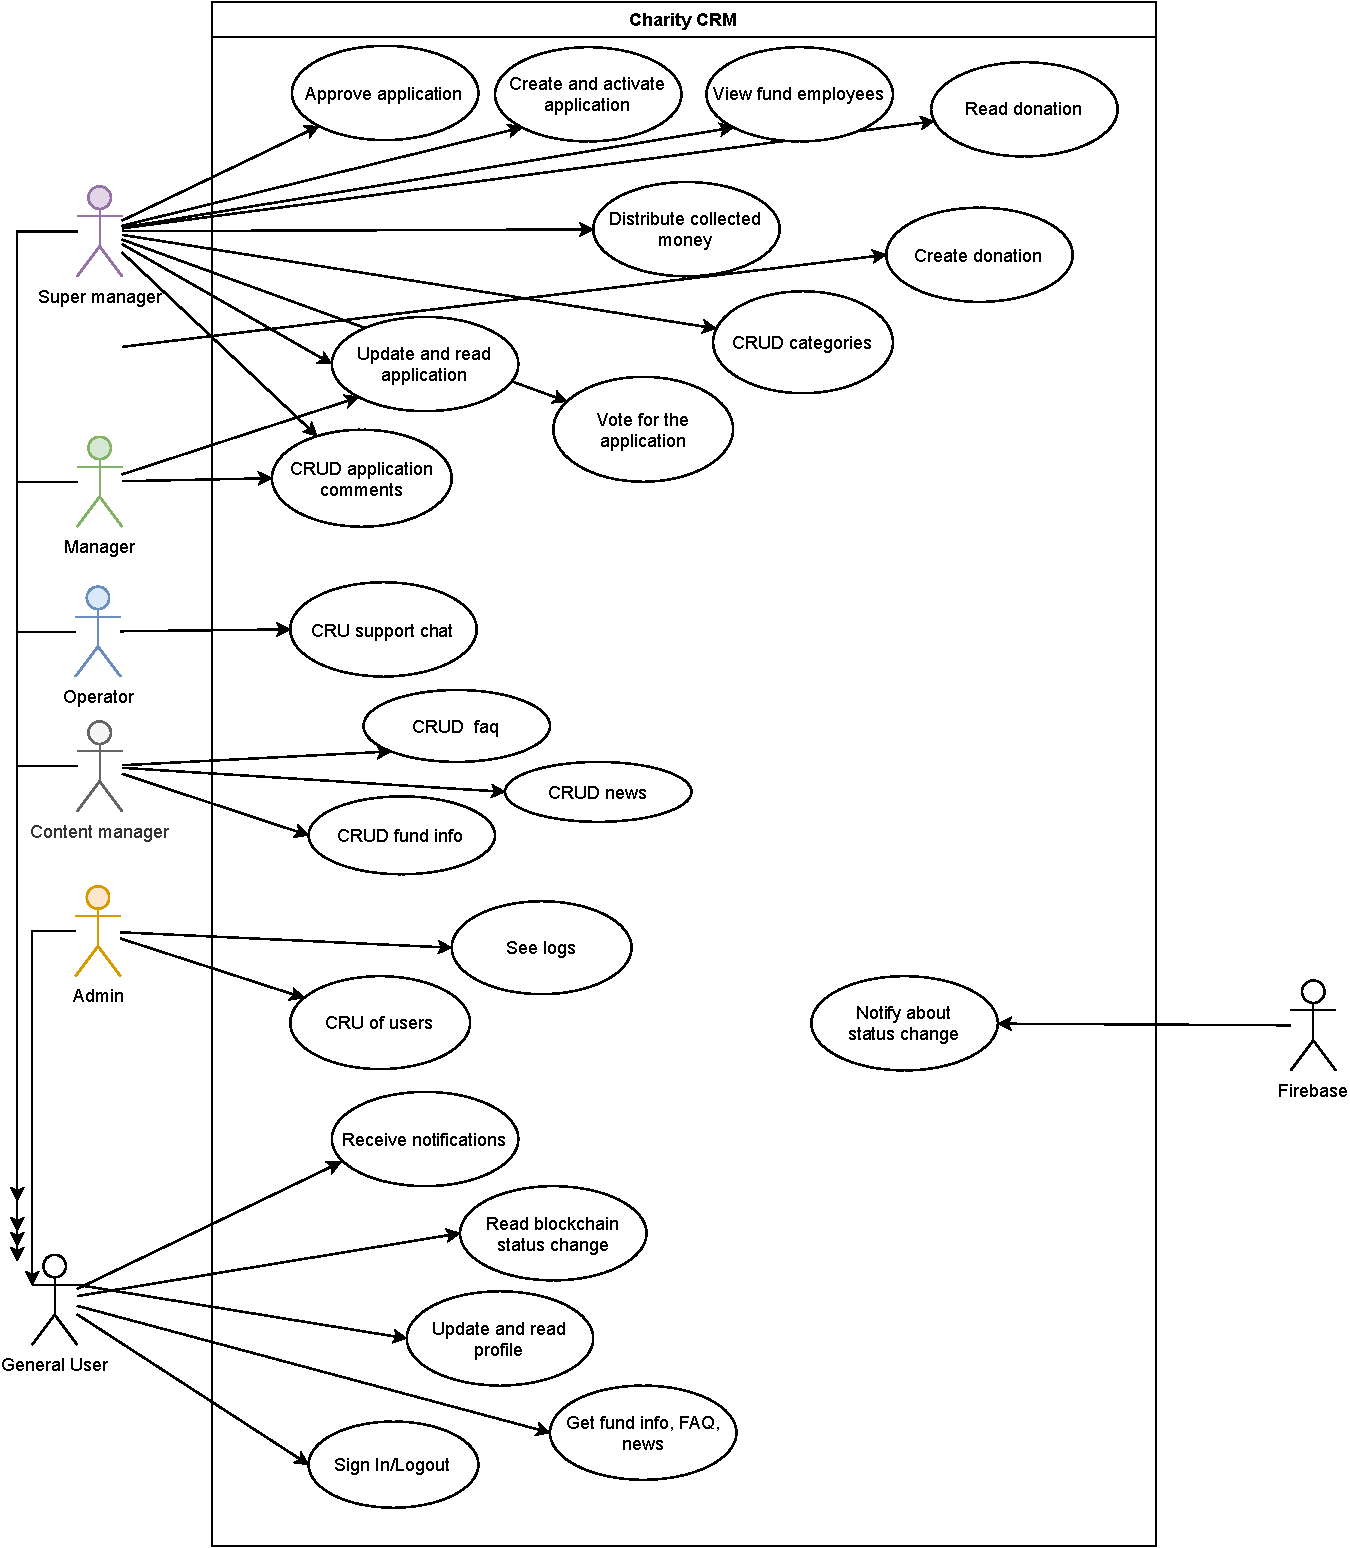
\includegraphics[width = 0.9\linewidth]{img/usecase.pdf}
		\caption{Диаграмма прецедентов}
		\label{pic: status}
	\end{figure}
	
	                    \newpage
	\addition{Диаграмма жизненного цикла заявки}{status} 
	
	\begin{figure}[H]
		\centering
		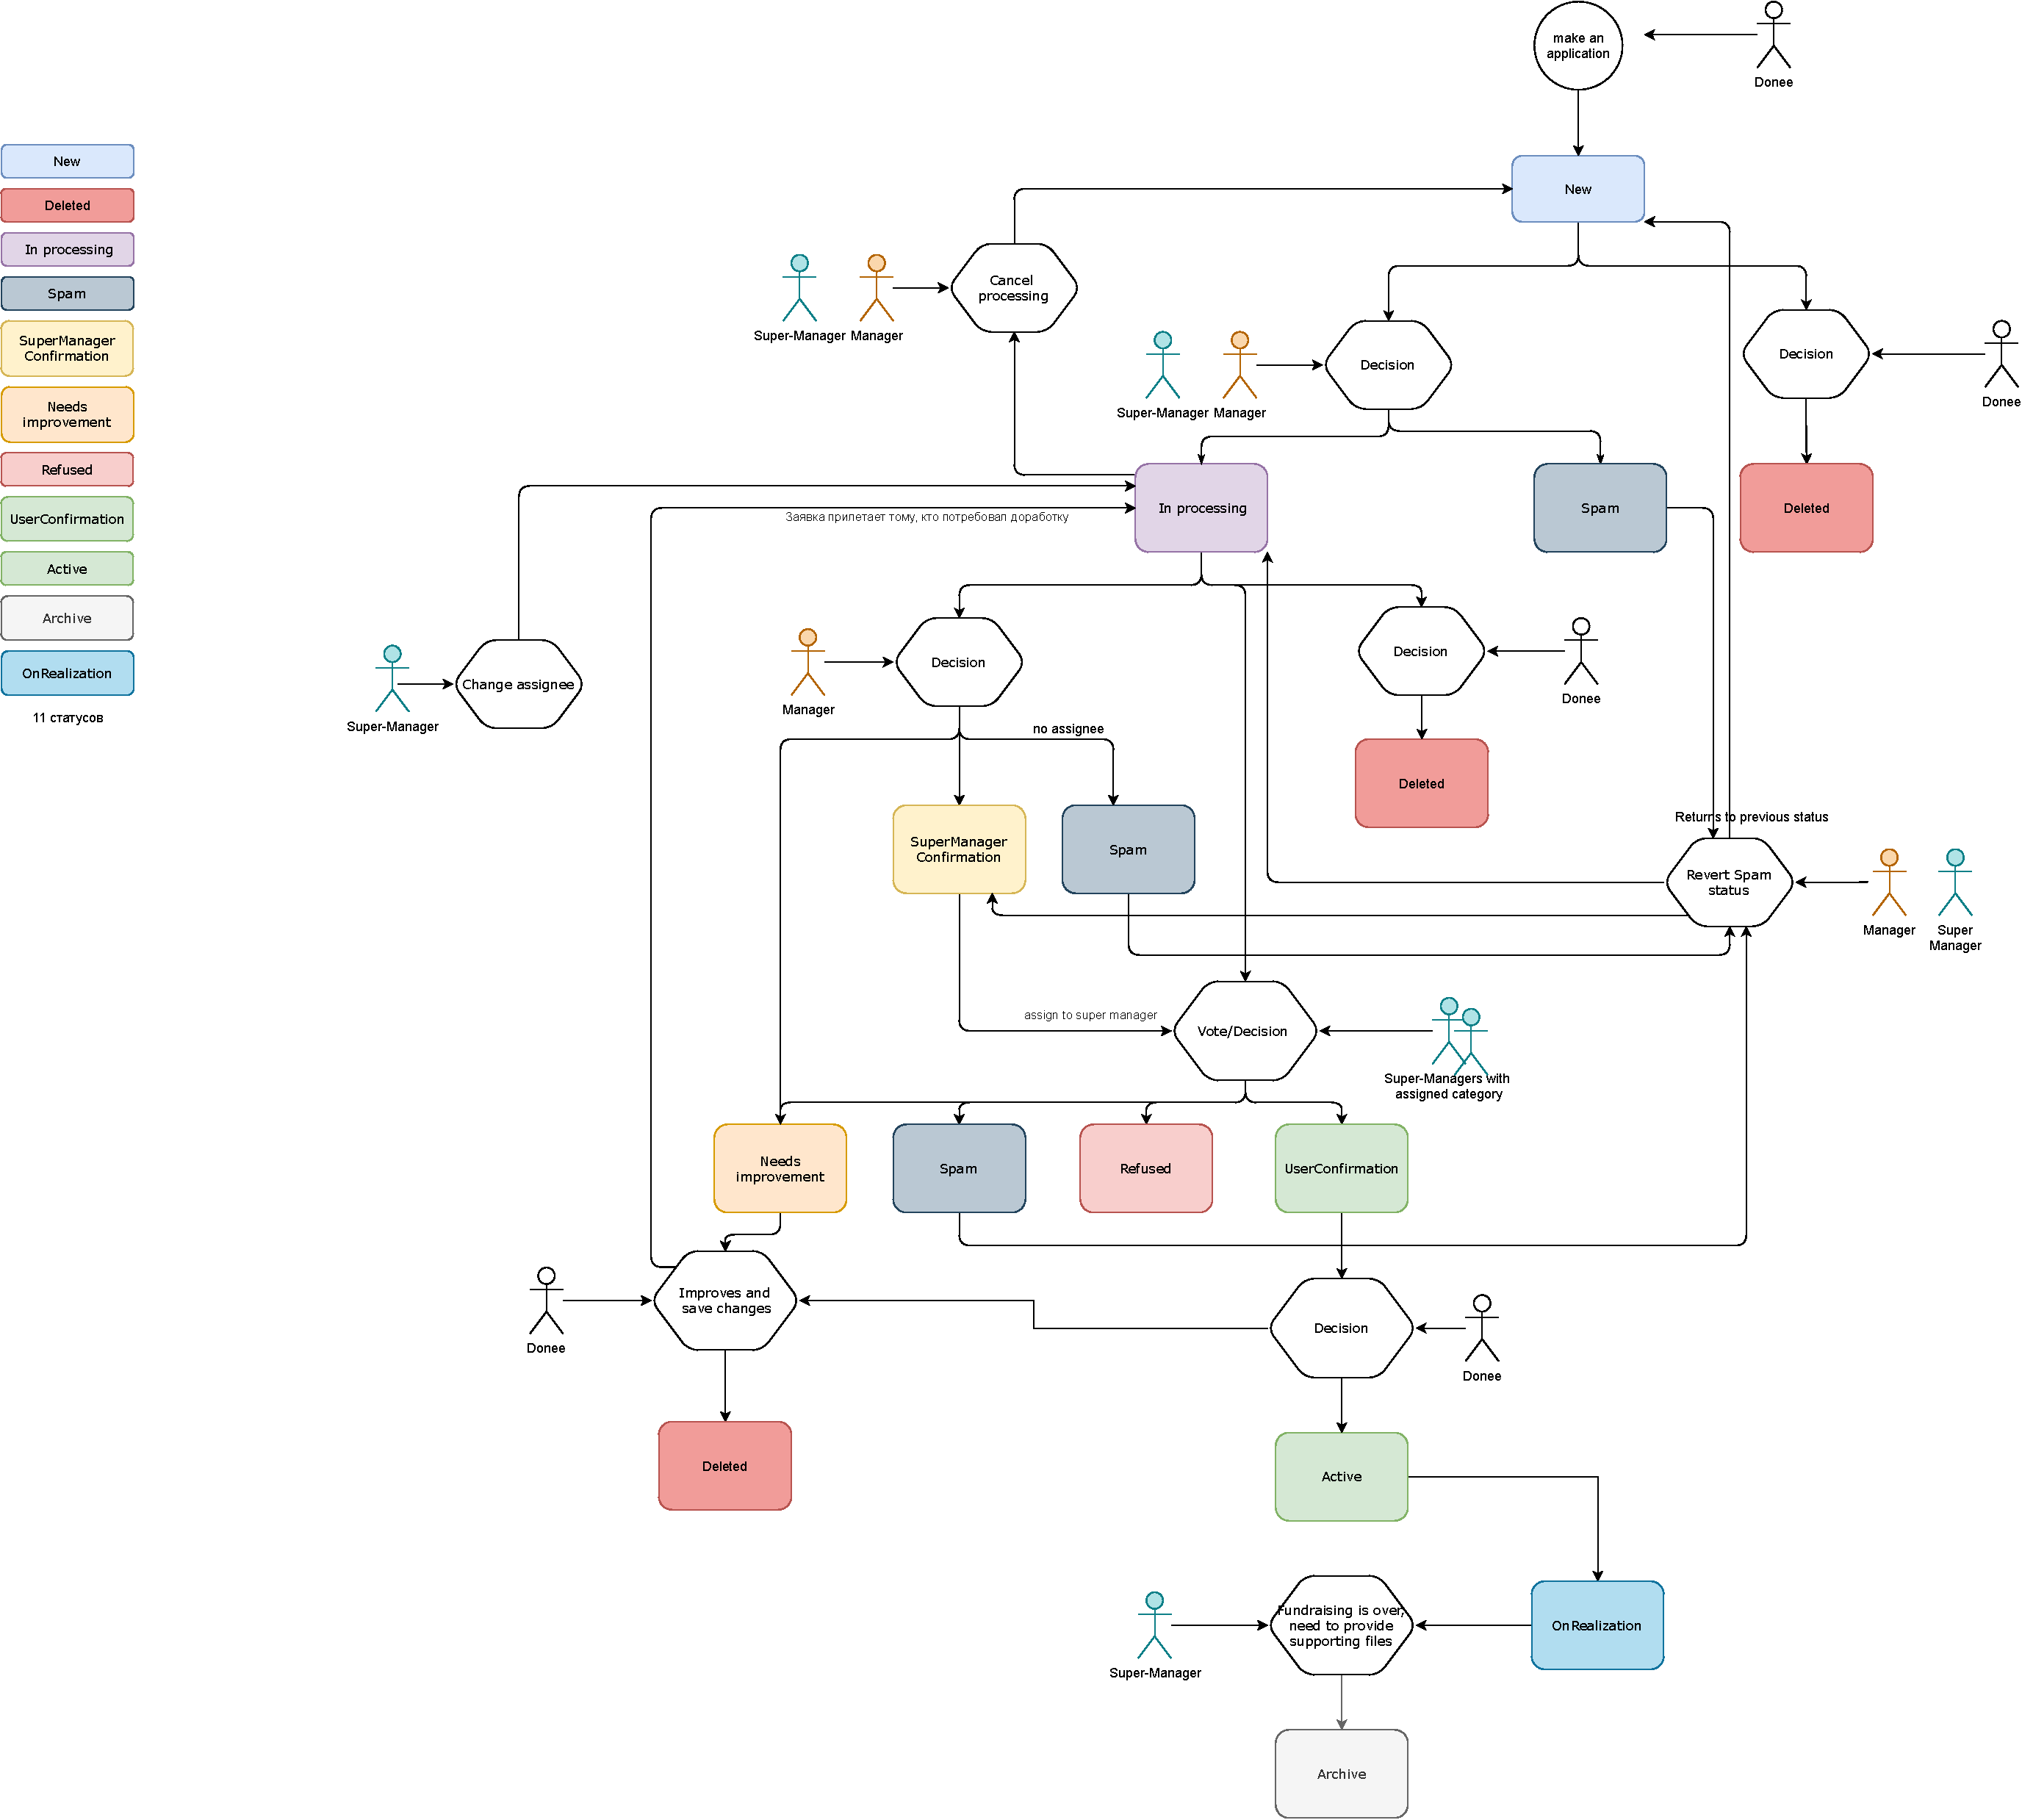
\includegraphics[width = 0.9\linewidth]{img/statusflow.pdf}
		\caption{Диаграмма статусов}
		\label{pic: status}
	\end{figure}
	
	\newpage
	\addition{Макеты интерфейса}{figma} 
	
	\begin{figure}[H]
		\centering
		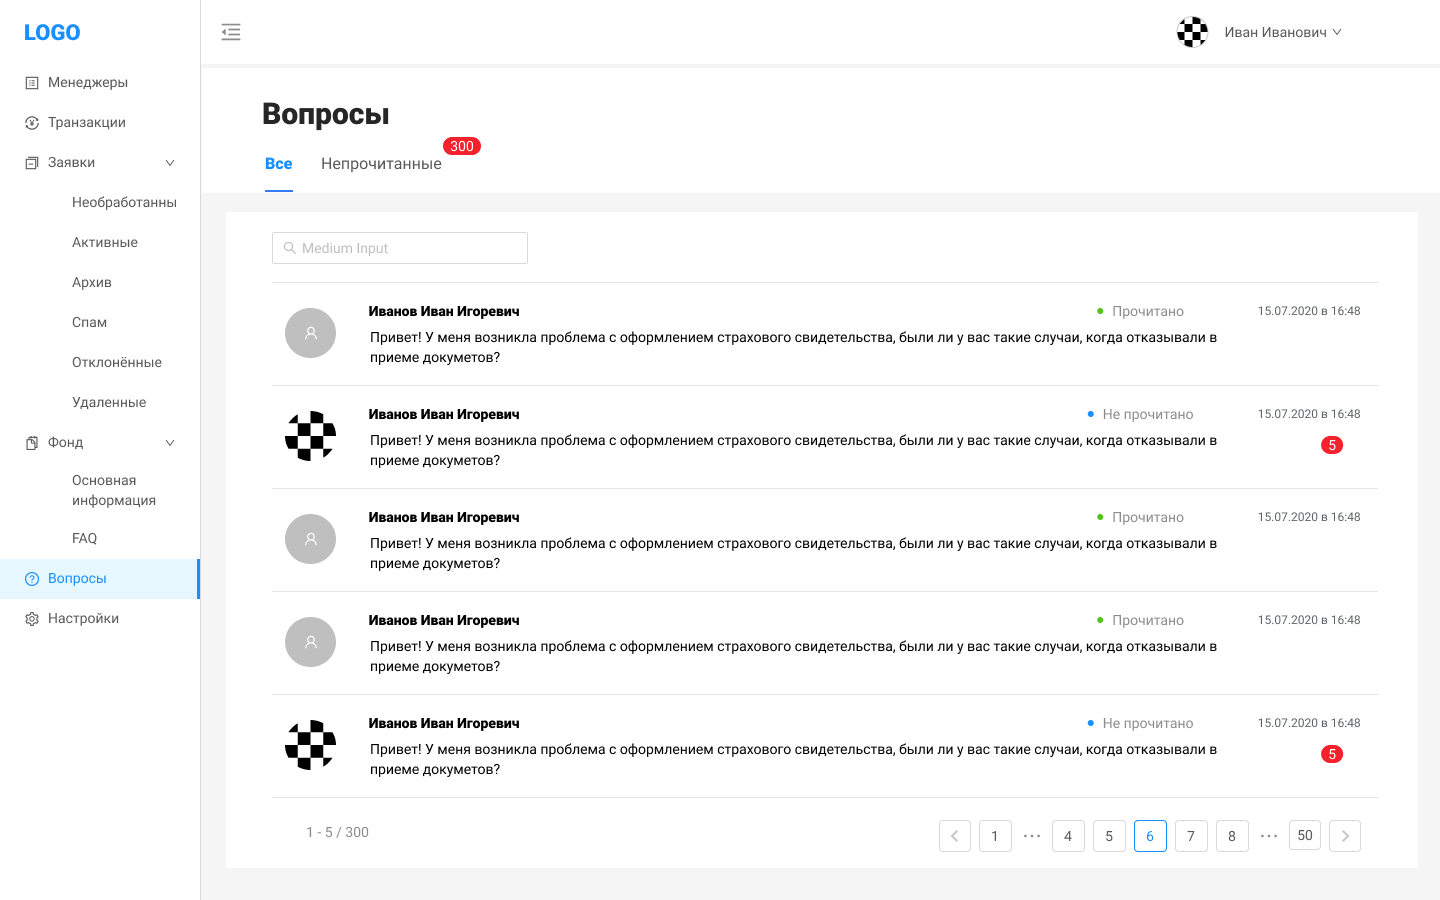
\includegraphics[width = 0.9\linewidth]{img/chats.png}
		\caption{Макет списка диалогов}
		\label{pic: applications}
\end{figure}

\begin{figure}[H]
		\centering
		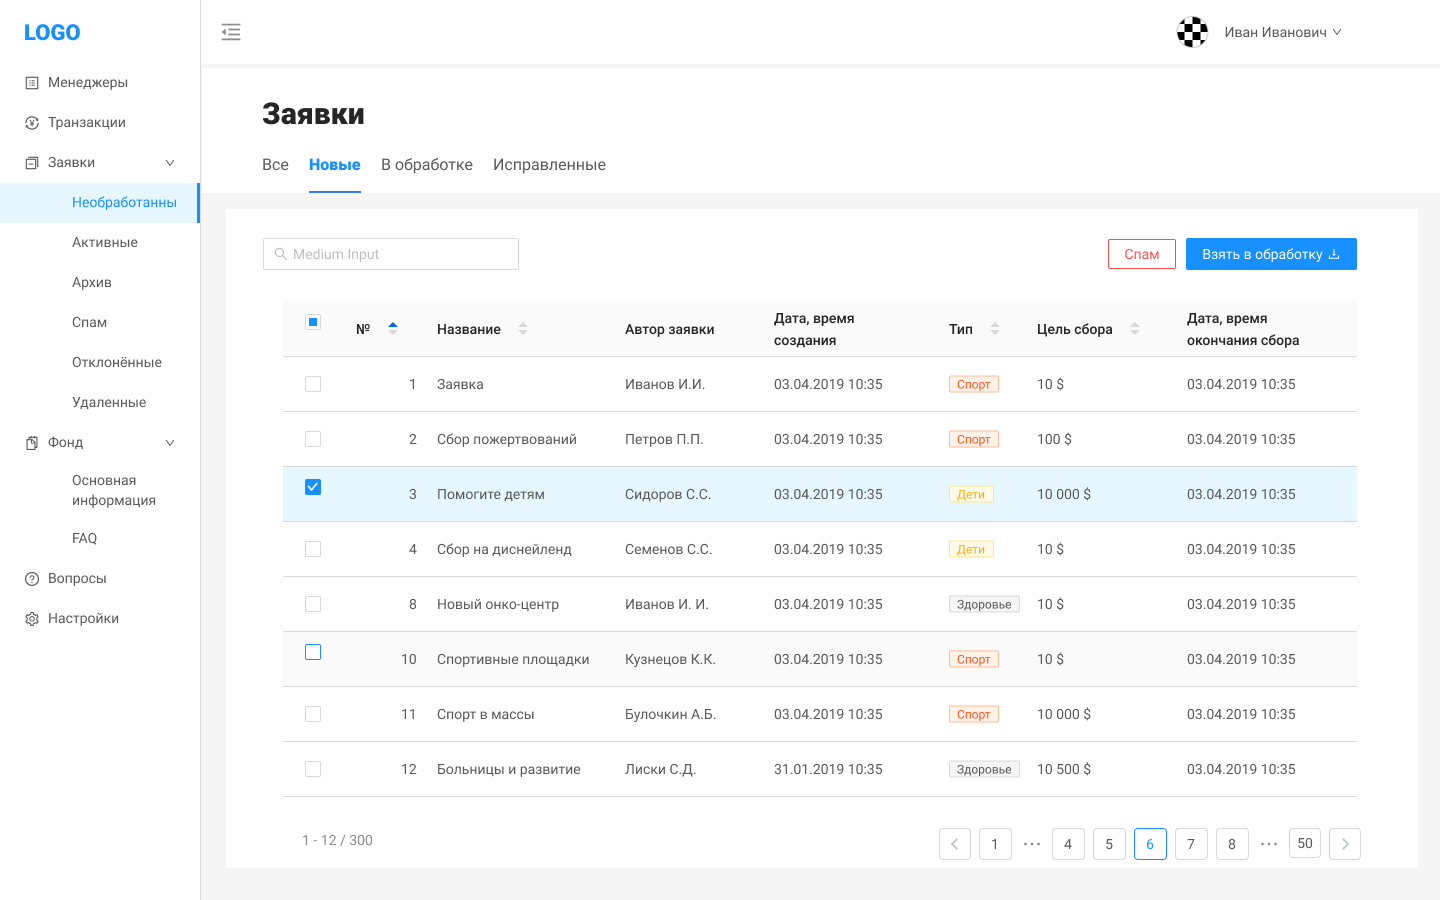
\includegraphics[width = 0.9\linewidth]{img/new.png}
		\caption{Макет списка заявок}
		\label{pic: applications}
\end{figure}

\begin{figure}[H]
		\centering
		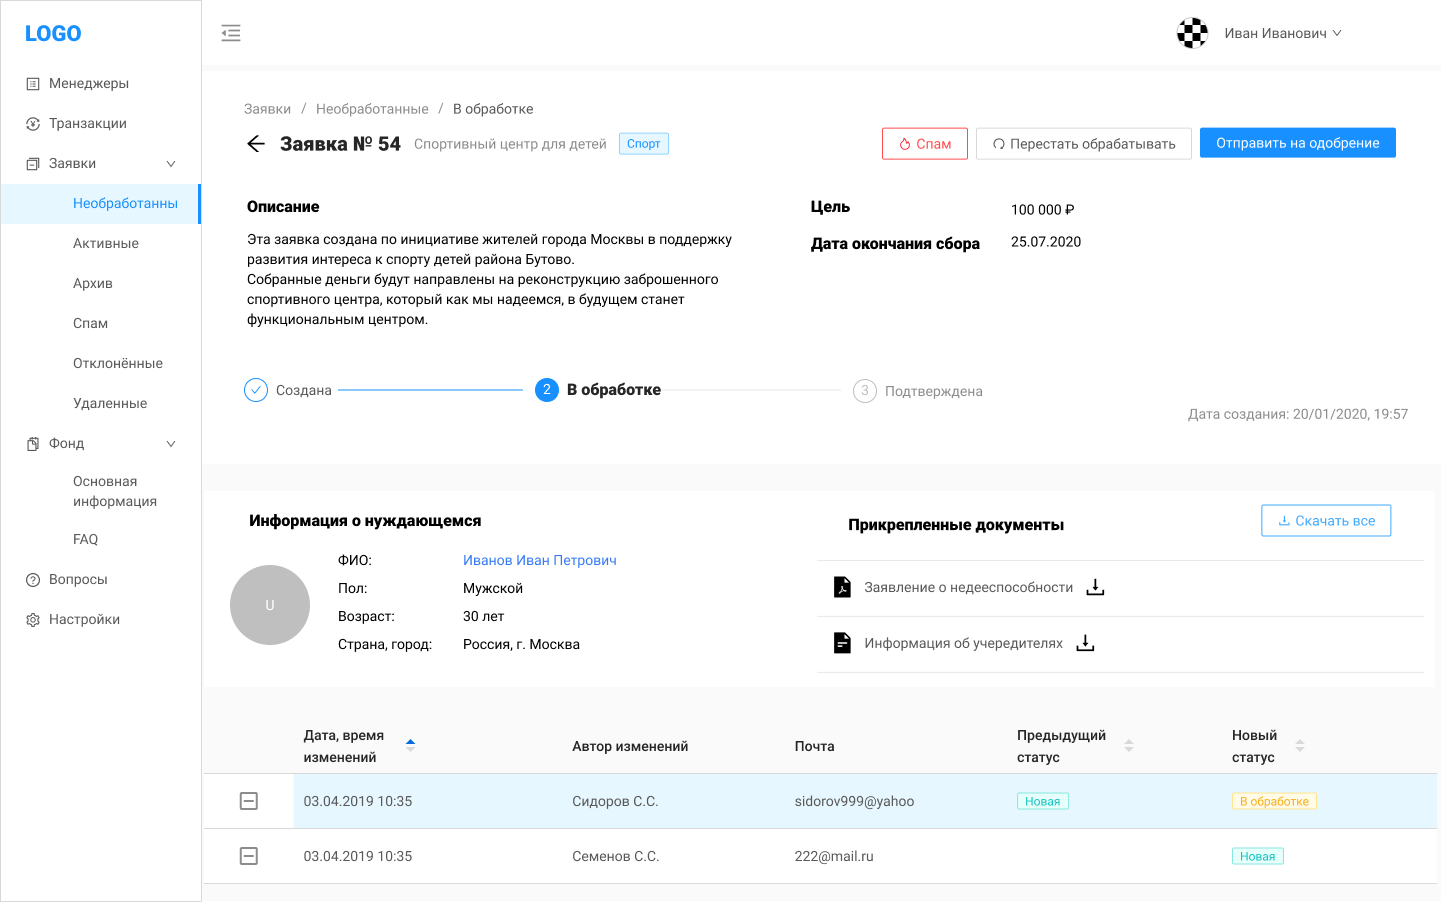
\includegraphics[width = 0.9\linewidth]{img/in-processing.png}
		\caption{Макет заявки}
		\label{pic: applications}
\end{figure}


						\newpage
	%\section{Источники, использованные при разработке}
	%\renewcommand{\refname}{Список источников}
	% \addcontentsline{toc}{subsection}{\refname}
	\patchcmd{\thebibliography}{\section*{\refname}}{}{}{}
	\anonsection{Список источников}
	\begin{thebibliography}{3}
		\bibitem{gost}Единая система программной документации – М.: ИПК, Издательство стандартов, 2000, 125 стр.
		\bibitem{lms} 
		LMS [Электронный ресурс] URL: 
		\url{https://lms.hse.ru} (Дата обращения: 16.11.2020, режим доступа: свободный)
		\bibitem{json} JSON [Электронный ресурс] URL: \url{https://www.json.org} (Дата обращения: 16.11.2020, режим доступа: свободный)
		\bibitem{md} Markdown Guide URL: \url{https://www.markdownguide.org} (Дата обращения: 16.04.2021).
		\bibitem{api} Swagger Charity API, v0.2 [Электронный ресурс] (Дата обращения: 31.05.2021, режим доступа: свободный) URL:\url{https://app.swaggerhub.com/apis/charity-crm/Charity/0.2}
	\end{thebibliography}

						\newpage
	\listRegistration

\end{document} % конец документа